% Options for packages loaded elsewhere
\PassOptionsToPackage{unicode}{hyperref}
\PassOptionsToPackage{hyphens}{url}
%
\documentclass[
]{book}
\usepackage{lmodern}
\usepackage{amssymb,amsmath}
\usepackage{ifxetex,ifluatex}
\ifnum 0\ifxetex 1\fi\ifluatex 1\fi=0 % if pdftex
  \usepackage[T1]{fontenc}
  \usepackage[utf8]{inputenc}
  \usepackage{textcomp} % provide euro and other symbols
\else % if luatex or xetex
  \usepackage{unicode-math}
  \defaultfontfeatures{Scale=MatchLowercase}
  \defaultfontfeatures[\rmfamily]{Ligatures=TeX,Scale=1}
\fi
% Use upquote if available, for straight quotes in verbatim environments
\IfFileExists{upquote.sty}{\usepackage{upquote}}{}
\IfFileExists{microtype.sty}{% use microtype if available
  \usepackage[]{microtype}
  \UseMicrotypeSet[protrusion]{basicmath} % disable protrusion for tt fonts
}{}
\makeatletter
\@ifundefined{KOMAClassName}{% if non-KOMA class
  \IfFileExists{parskip.sty}{%
    \usepackage{parskip}
  }{% else
    \setlength{\parindent}{0pt}
    \setlength{\parskip}{6pt plus 2pt minus 1pt}}
}{% if KOMA class
  \KOMAoptions{parskip=half}}
\makeatother
\usepackage{xcolor}
\IfFileExists{xurl.sty}{\usepackage{xurl}}{} % add URL line breaks if available
\IfFileExists{bookmark.sty}{\usepackage{bookmark}}{\usepackage{hyperref}}
\hypersetup{
  pdftitle={Team collaboration and management softwares},
  pdfauthor={Team Even Better},
  hidelinks,
  pdfcreator={LaTeX via pandoc}}
\urlstyle{same} % disable monospaced font for URLs
\usepackage{color}
\usepackage{fancyvrb}
\newcommand{\VerbBar}{|}
\newcommand{\VERB}{\Verb[commandchars=\\\{\}]}
\DefineVerbatimEnvironment{Highlighting}{Verbatim}{commandchars=\\\{\}}
% Add ',fontsize=\small' for more characters per line
\usepackage{framed}
\definecolor{shadecolor}{RGB}{248,248,248}
\newenvironment{Shaded}{\begin{snugshade}}{\end{snugshade}}
\newcommand{\AlertTok}[1]{\textcolor[rgb]{0.94,0.16,0.16}{#1}}
\newcommand{\AnnotationTok}[1]{\textcolor[rgb]{0.56,0.35,0.01}{\textbf{\textit{#1}}}}
\newcommand{\AttributeTok}[1]{\textcolor[rgb]{0.77,0.63,0.00}{#1}}
\newcommand{\BaseNTok}[1]{\textcolor[rgb]{0.00,0.00,0.81}{#1}}
\newcommand{\BuiltInTok}[1]{#1}
\newcommand{\CharTok}[1]{\textcolor[rgb]{0.31,0.60,0.02}{#1}}
\newcommand{\CommentTok}[1]{\textcolor[rgb]{0.56,0.35,0.01}{\textit{#1}}}
\newcommand{\CommentVarTok}[1]{\textcolor[rgb]{0.56,0.35,0.01}{\textbf{\textit{#1}}}}
\newcommand{\ConstantTok}[1]{\textcolor[rgb]{0.00,0.00,0.00}{#1}}
\newcommand{\ControlFlowTok}[1]{\textcolor[rgb]{0.13,0.29,0.53}{\textbf{#1}}}
\newcommand{\DataTypeTok}[1]{\textcolor[rgb]{0.13,0.29,0.53}{#1}}
\newcommand{\DecValTok}[1]{\textcolor[rgb]{0.00,0.00,0.81}{#1}}
\newcommand{\DocumentationTok}[1]{\textcolor[rgb]{0.56,0.35,0.01}{\textbf{\textit{#1}}}}
\newcommand{\ErrorTok}[1]{\textcolor[rgb]{0.64,0.00,0.00}{\textbf{#1}}}
\newcommand{\ExtensionTok}[1]{#1}
\newcommand{\FloatTok}[1]{\textcolor[rgb]{0.00,0.00,0.81}{#1}}
\newcommand{\FunctionTok}[1]{\textcolor[rgb]{0.00,0.00,0.00}{#1}}
\newcommand{\ImportTok}[1]{#1}
\newcommand{\InformationTok}[1]{\textcolor[rgb]{0.56,0.35,0.01}{\textbf{\textit{#1}}}}
\newcommand{\KeywordTok}[1]{\textcolor[rgb]{0.13,0.29,0.53}{\textbf{#1}}}
\newcommand{\NormalTok}[1]{#1}
\newcommand{\OperatorTok}[1]{\textcolor[rgb]{0.81,0.36,0.00}{\textbf{#1}}}
\newcommand{\OtherTok}[1]{\textcolor[rgb]{0.56,0.35,0.01}{#1}}
\newcommand{\PreprocessorTok}[1]{\textcolor[rgb]{0.56,0.35,0.01}{\textit{#1}}}
\newcommand{\RegionMarkerTok}[1]{#1}
\newcommand{\SpecialCharTok}[1]{\textcolor[rgb]{0.00,0.00,0.00}{#1}}
\newcommand{\SpecialStringTok}[1]{\textcolor[rgb]{0.31,0.60,0.02}{#1}}
\newcommand{\StringTok}[1]{\textcolor[rgb]{0.31,0.60,0.02}{#1}}
\newcommand{\VariableTok}[1]{\textcolor[rgb]{0.00,0.00,0.00}{#1}}
\newcommand{\VerbatimStringTok}[1]{\textcolor[rgb]{0.31,0.60,0.02}{#1}}
\newcommand{\WarningTok}[1]{\textcolor[rgb]{0.56,0.35,0.01}{\textbf{\textit{#1}}}}
\usepackage{longtable,booktabs}
% Correct order of tables after \paragraph or \subparagraph
\usepackage{etoolbox}
\makeatletter
\patchcmd\longtable{\par}{\if@noskipsec\mbox{}\fi\par}{}{}
\makeatother
% Allow footnotes in longtable head/foot
\IfFileExists{footnotehyper.sty}{\usepackage{footnotehyper}}{\usepackage{footnote}}
\makesavenoteenv{longtable}
\usepackage{graphicx,grffile}
\makeatletter
\def\maxwidth{\ifdim\Gin@nat@width>\linewidth\linewidth\else\Gin@nat@width\fi}
\def\maxheight{\ifdim\Gin@nat@height>\textheight\textheight\else\Gin@nat@height\fi}
\makeatother
% Scale images if necessary, so that they will not overflow the page
% margins by default, and it is still possible to overwrite the defaults
% using explicit options in \includegraphics[width, height, ...]{}
\setkeys{Gin}{width=\maxwidth,height=\maxheight,keepaspectratio}
% Set default figure placement to htbp
\makeatletter
\def\fps@figure{htbp}
\makeatother
\setlength{\emergencystretch}{3em} % prevent overfull lines
\providecommand{\tightlist}{%
  \setlength{\itemsep}{0pt}\setlength{\parskip}{0pt}}
\setcounter{secnumdepth}{5}
\usepackage{booktabs}
\usepackage[]{natbib}
\bibliographystyle{plainnat}

\title{Team collaboration and management softwares}
\author{Team Even Better}
\date{2022-07-25}

\begin{document}
\maketitle

{
\setcounter{tocdepth}{1}
\tableofcontents
}
\hypertarget{about}{%
\chapter{About}\label{about}}

This is a \emph{Team collaboration and management softwares} book written in \textbf{Markdown}.

\hypertarget{usage}{%
\section{Usage}\label{usage}}

Each \textbf{bookdown} chapter is an .Rmd file, and each .Rmd file can contain one (and only one) chapter. A chapter \emph{must} start with a first-level heading: \texttt{\#\ A\ good\ chapter}, and can contain one (and only one) first-level heading.

Use second-level and higher headings within chapters like: \texttt{\#\#\ A\ short\ section} or \texttt{\#\#\#\ An\ even\ shorter\ section}.

The \texttt{index.Rmd} file is required, and is also your first book chapter. It will be the homepage when you render the book.

\hypertarget{render-book}{%
\section{Render book}\label{render-book}}

You can render the HTML version of this example book without changing anything:

\begin{enumerate}
\def\labelenumi{\arabic{enumi}.}
\item
  Find the \textbf{Build} pane in the RStudio IDE, and
\item
  Click on \textbf{Build Book}, then select your output format, or select ``All formats'' if you'd like to use multiple formats from the same book source files.
\end{enumerate}

Or build the book from the R console:

\begin{Shaded}
\begin{Highlighting}[]
\NormalTok{bookdown}\OperatorTok{::}\KeywordTok{render_book}\NormalTok{()}
\end{Highlighting}
\end{Shaded}

To render this example to PDF as a \texttt{bookdown::pdf\_book}, you'll need to install XeLaTeX. You are recommended to install TinyTeX (which includes XeLaTeX): \url{https://yihui.org/tinytex/}.

\hypertarget{preview-book}{%
\section{Preview book}\label{preview-book}}

As you work, you may start a local server to live preview this HTML book. This preview will update as you edit the book when you save individual .Rmd files. You can start the server in a work session by using the RStudio add-in ``Preview book'', or from the R console:

\begin{Shaded}
\begin{Highlighting}[]
\NormalTok{bookdown}\OperatorTok{::}\KeywordTok{serve_book}\NormalTok{()}
\end{Highlighting}
\end{Shaded}

\hypertarget{introduction}{%
\chapter{Introduction}\label{introduction}}

We plan on making a guide for future MBAn students focused on team collaboration and management software that may be used for team projects. The guide will include three parts: an introductory overview of the contents of our guide, a detailed breakdown of the tools that we have selected to cover, and a final summary of user feedback and suggestions by current MBAn students.

Below, you will find a preliminary breakdown of the structure of our guide, including the different software/platforms that we plan to cover. For each of the chosen collaboration tools, we plan on providing the following information: an introduction, the main features, and who tends to use the tool. We have also selected one tool from each of four categories, as shown in bold, to provide more detailed information on, which will include a detailed tutorial on installation, how to use the main features, how to troubleshoot common problems, and more.

\hypertarget{about-us}{%
\chapter{About us}\label{about-us}}

\hypertarget{tong-su}{%
\section{Tong Su}\label{tong-su}}

\begin{figure}

\includegraphics[width=0.2\linewidth,height=0.2\textheight]{tong} \caption{This is me!}\label{fig:unnamed-chunk-4}
\end{figure}

\begin{itemize}
\item
  Name: \textbf{Tong Su}
\item
  Email: \href{mailto:sutongln@umich.edu}{\nolinkurl{sutongln@umich.edu}}
\item
  Education:

  \begin{itemize}
  \item
    University of Michigan, Master of Business Analytics, Apr 2023
  \item
    Sun Yat-sen University, Bachelor of Finance, Jun 2020
  \end{itemize}
\item
  Hobbies: Musics, Movies, Swimming, Traveling
\item
  1 Fun Fact: I was the cheerleader of my college at my undergraduate school.
\end{itemize}

\hypertarget{lida-zhang}{%
\section{Lida Zhang}\label{lida-zhang}}

\begin{figure}
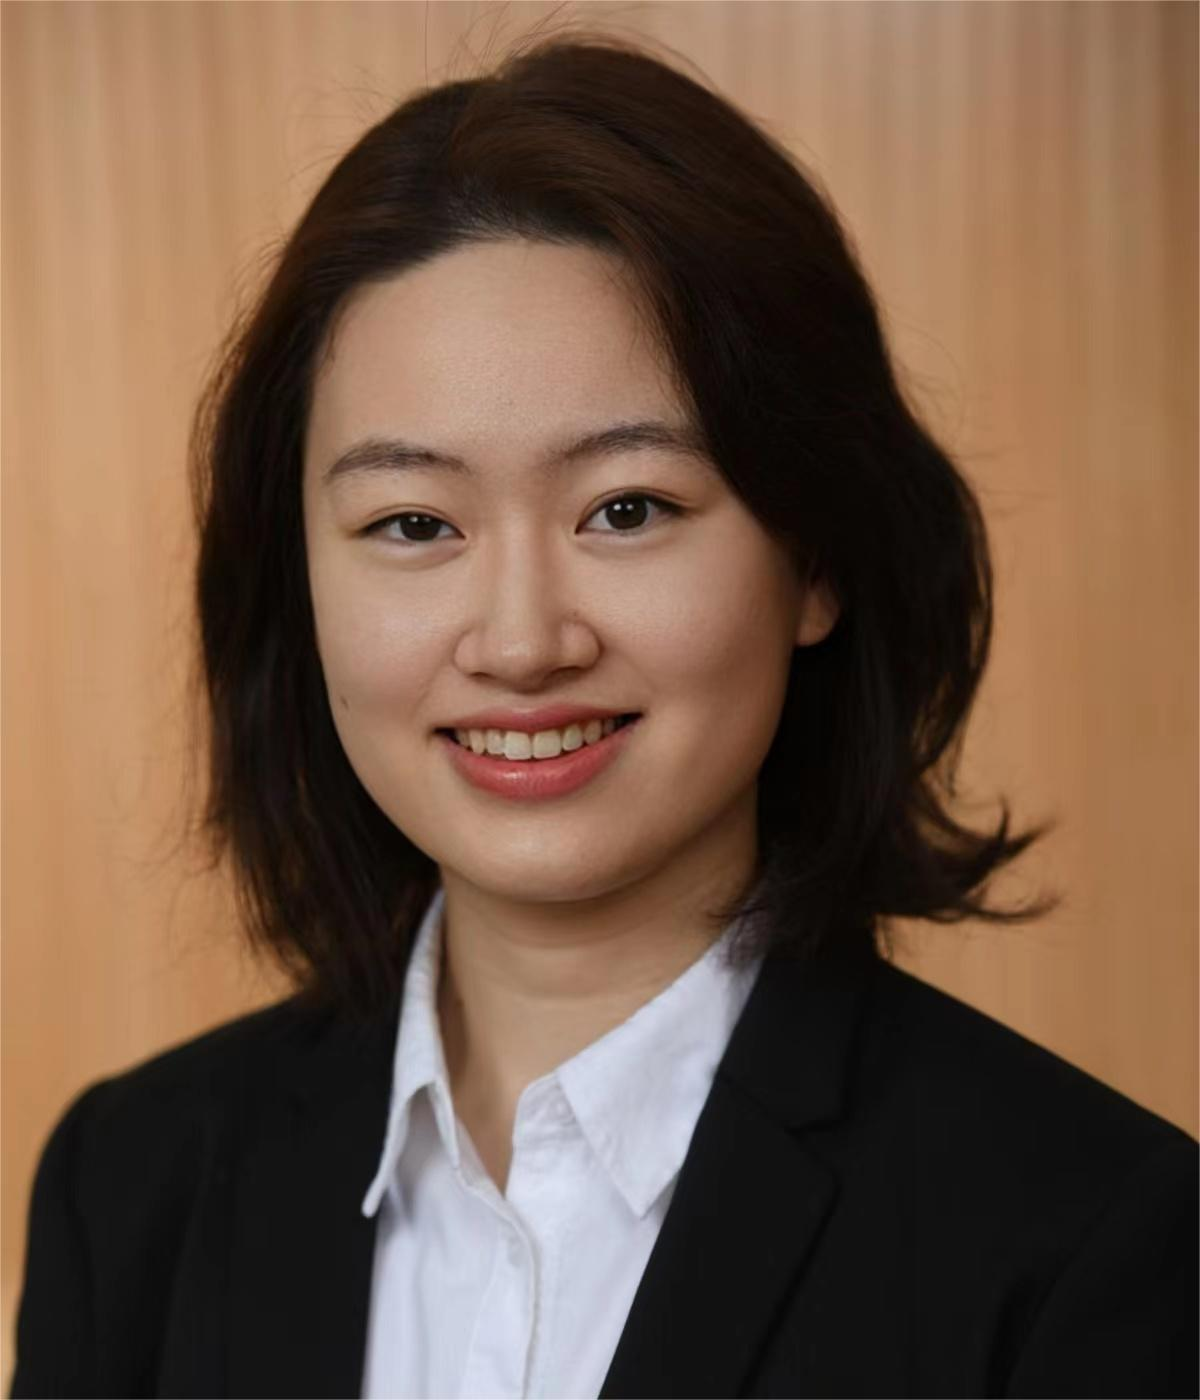
\includegraphics[width=0.2\linewidth,height=0.2\textheight]{img_lida} \caption{This is me!}\label{fig:unnamed-chunk-5}
\end{figure}

\begin{itemize}
\item
  Name: \textbf{Lida Zhang}
\item
  Email: \href{mailto:lidazh@umich.edu}{\nolinkurl{lidazh@umich.edu}}
\item
  Education:

  \begin{itemize}
  \item
    University of Michigan, Master of Business Analytics, Apr 2023
  \item
    Shanghai University of Finance and Economics, Bachelor of Mathematical Economics, Jun 2021
  \end{itemize}
\item
  Hobbies: Traveling, Jogging, Badminton, Yoga
\item
  1 Fun Fact: I have traveled to 15 countries in 4 continents including Middle East, Western Europe, and New Zealand
\end{itemize}

\hypertarget{lilia-bei}{%
\section{Lilia Bei}\label{lilia-bei}}

\begin{figure}
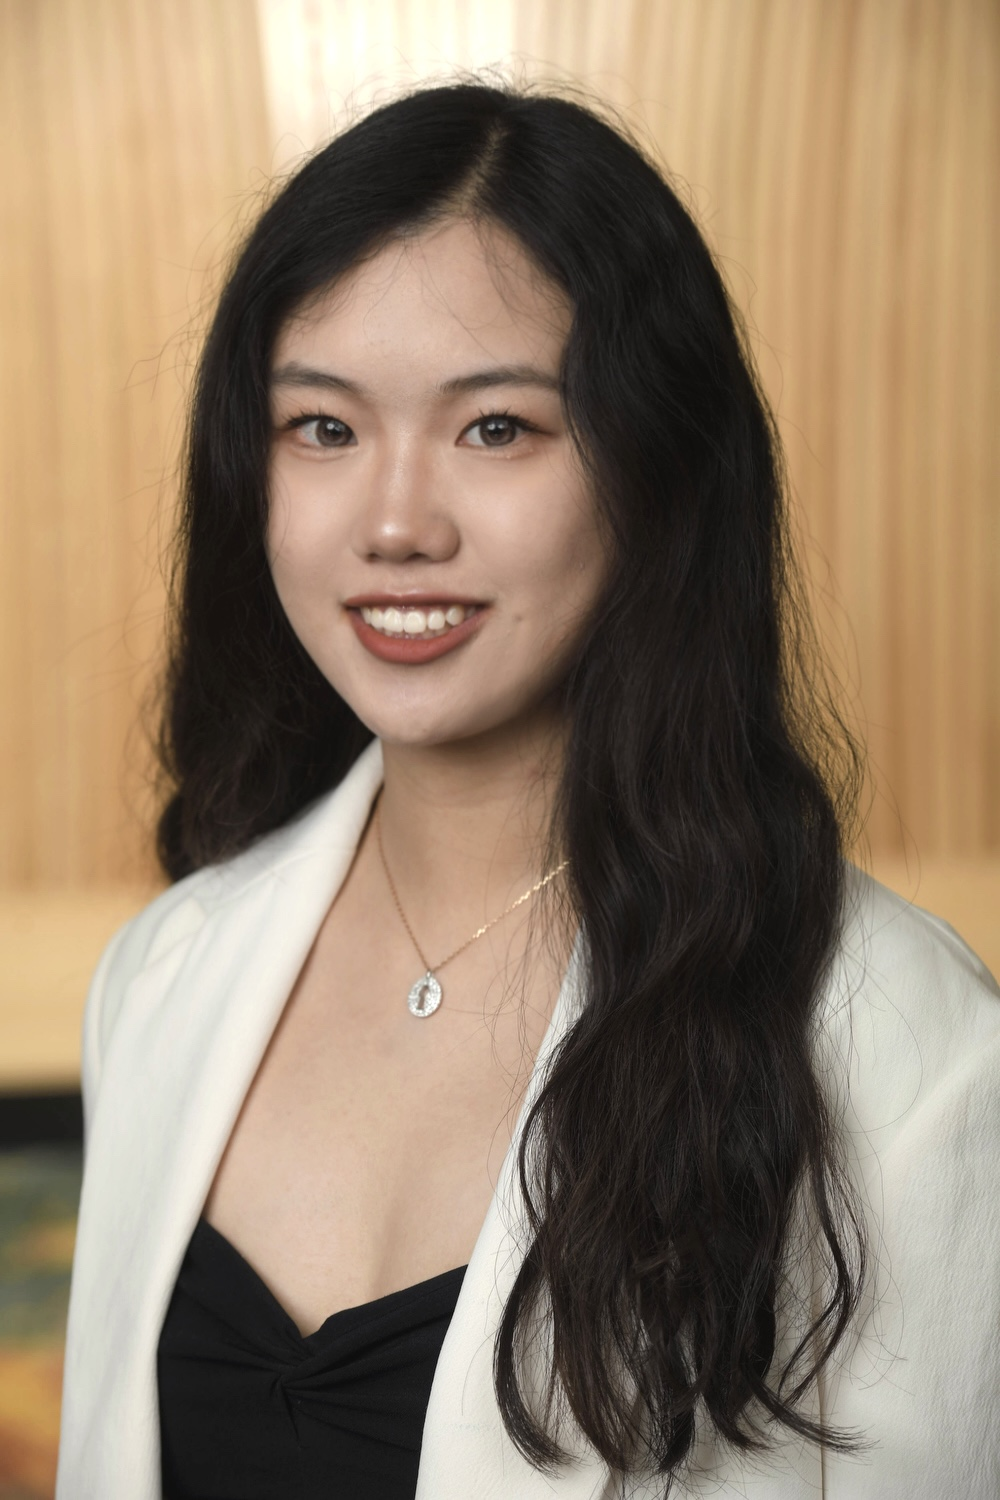
\includegraphics[width=0.2\linewidth,height=0.2\textheight]{lilia} \caption{This is me!}\label{fig:unnamed-chunk-6}
\end{figure}

\begin{itemize}
\item
  Name: \textbf{Lilia Bei}
\item
  Email: \href{mailto:yangbei@umich.edu}{\nolinkurl{yangbei@umich.edu}}
\item
  Education:

  \begin{itemize}
  \item
    University of Michigan, Master of Business Analytics, Apr 2023
  \item
    University of Michigan, B.A. in Communication and Media, Apr 2022
  \end{itemize}
\item
  Hobbies: movies, music, tennis, shopping
\item
  1 Fun Fact: I am afraid of cats, especially black cats, and balloons (because of the popping sound)
\end{itemize}

\hypertarget{yining-zheng}{%
\section{Yining Zheng}\label{yining-zheng}}

\begin{figure}

\includegraphics[width=0.2\linewidth,height=0.2\textheight]{Yining} \caption{This is me!}\label{fig:unnamed-chunk-7}
\end{figure}

\begin{itemize}
\item
  Name: \textbf{Yining Zheng}
\item
  Email: \href{mailto:haileyz@umich.edu}{\nolinkurl{haileyz@umich.edu}}
\item
  Education:

  \begin{itemize}
  \item
    University of Michigan, Master of Business Analytics, Apr 2023
  \item
    BNU-HKBU United International College, Bachelor of Accounting, Jun 2022
  \end{itemize}
\item
  Hobbies: Swimming, Traveling, Shopping, Sleeping
\item
  1 Fun Fact: Thrill-seeking, like watching horror movies, going to haunted houses, and wanting to try bungee jumping and skydiving.
\end{itemize}

\hypertarget{nilsa-ileana-pedanou}{%
\section{Nilsa Ileana Pedanou}\label{nilsa-ileana-pedanou}}

\begin{figure}
\includegraphics[width=0.2\linewidth,height=0.2\textheight]{Nilsa} \caption{This is me!}\label{fig:unnamed-chunk-8}
\end{figure}

\begin{itemize}
\item
  Name: \textbf{Nilsa Ileana Pedanou}
\item
  Email: \href{mailto:npedanou@umich.edu}{\nolinkurl{npedanou@umich.edu}}
\item
  Education:

  \begin{itemize}
  \item
    University of Michigan, Master of Business Analytics, Apr 2023
  \item
    University of Michigan, Bachelor of Science in Engineering - Chemical Engineering, Apr 2022
  \end{itemize}
\item
  Hobbies: Baking, Working Out, Sleeping, Puzzles, Talking with Family
\item
  1 Fun Fact: I have very vivid dreams, and I one day hope to make a movie about one!
\end{itemize}

\hypertarget{overview}{%
\chapter{Overview}\label{overview}}

\hypertarget{the-common-form-of-team-activity-in-mban}{%
\section{The common form of team activity in MBAn}\label{the-common-form-of-team-activity-in-mban}}

The common form of team activity in MBAn

\hypertarget{the-importance-of-team-collaboration}{%
\section{The importance of team collaboration}\label{the-importance-of-team-collaboration}}

The importance of team collaboration

\hypertarget{the-importance-of-increasing-efficiency-of-teamwork}{%
\section{The importance of increasing efficiency of teamwork}\label{the-importance-of-increasing-efficiency-of-teamwork}}

The importance of increasing efficiency of teamwork

\hypertarget{the-convenience-of-the-team-collaboration-tool}{%
\section{The convenience of the team collaboration tool}\label{the-convenience-of-the-team-collaboration-tool}}

The convenience of the team collaboration tool

\hypertarget{tools-for-documentation-and-file-sharing}{%
\chapter{Tools for documentation and file sharing}\label{tools-for-documentation-and-file-sharing}}

You can add parts to organize one or more book chapters together. Parts can be inserted at the top of an .Rmd file, before the first-level chapter heading in that same file.

Add a numbered part: \texttt{\#\ (PART)\ Act\ one\ \{-\}} (followed by \texttt{\#\ A\ chapter})

Add an unnumbered part: \texttt{\#\ (PART\textbackslash{}*)\ Act\ one\ \{-\}} (followed by \texttt{\#\ A\ chapter})

Add an appendix as a special kind of un-numbered part: \texttt{\#\ (APPENDIX)\ Other\ stuff\ \{-\}} (followed by \texttt{\#\ A\ chapter}). Chapters in an appendix are prepended with letters instead of numbers.

\hypertarget{google-suitedrivedocssheetsslides}{%
\section{Google Suite(Drive/Docs/Sheets/Slides)}\label{google-suitedrivedocssheetsslides}}

All chapter sections start with a second-level (\texttt{\#\#}) or higher heading followed by your section title, like the sections above and below here. You can have as many as you want within a chapter.

\hypertarget{introduction-1}{%
\subsection{Introduction}\label{introduction-1}}

Chapters and sections are numbered by default. To un-number a heading, add a \texttt{\{.unnumbered\}} or the shorter \texttt{\{-\}} at the end of the heading, like in this section.

\hypertarget{main-features}{%
\subsection{Main features}\label{main-features}}

\hypertarget{who-tends-to-love-it}{%
\subsection{Who tends to love it?}\label{who-tends-to-love-it}}

\hypertarget{tutorial}{%
\subsection{Tutorial}\label{tutorial}}

\hypertarget{dropbox}{%
\section{Dropbox}\label{dropbox}}

\hypertarget{introduction-2}{%
\subsection{Introduction}\label{introduction-2}}

Chapters and sections are numbered by default. To un-number a heading, add a \texttt{\{.unnumbered\}} or the shorter \texttt{\{-\}} at the end of the heading, like in this section.

\hypertarget{main-features-1}{%
\subsection{Main features}\label{main-features-1}}

\hypertarget{who-tends-to-love-it-1}{%
\subsection{Who tends to love it?}\label{who-tends-to-love-it-1}}

\hypertarget{tools-for-programming}{%
\chapter{Tools for programming}\label{tools-for-programming}}

\hypertarget{github}{%
\section{Github}\label{github}}

\hypertarget{introduction-3}{%
\subsection{Introduction}\label{introduction-3}}

\hypertarget{main-features-2}{%
\subsection{Main features}\label{main-features-2}}

\hypertarget{who-tends-to-love-it-2}{%
\subsection{Who tends to love it?}\label{who-tends-to-love-it-2}}

\hypertarget{tutorial-1}{%
\subsection{Tutorial}\label{tutorial-1}}

\hypertarget{colab}{%
\section{Colab}\label{colab}}

\hypertarget{introduction-4}{%
\subsection{Introduction}\label{introduction-4}}

\hypertarget{main-features-3}{%
\subsection{Main features}\label{main-features-3}}

\hypertarget{who-tends-to-love-it-3}{%
\subsection{Who tends to love it?}\label{who-tends-to-love-it-3}}

\hypertarget{tools-for-messaging-and-virtual-meeting}{%
\chapter{Tools for messaging and virtual meeting}\label{tools-for-messaging-and-virtual-meeting}}

\hypertarget{zoom}{%
\section{Zoom}\label{zoom}}

\hypertarget{introduction-5}{%
\subsection{Introduction}\label{introduction-5}}

\hypertarget{main-features-4}{%
\subsection{Main features}\label{main-features-4}}

\hypertarget{who-tends-to-love-it-4}{%
\subsection{Who tends to love it?}\label{who-tends-to-love-it-4}}

\hypertarget{tutorial-2}{%
\subsection{Tutorial}\label{tutorial-2}}

\hypertarget{groupme}{%
\section{GroupMe}\label{groupme}}

\hypertarget{introduction-6}{%
\subsection{Introduction}\label{introduction-6}}

\hypertarget{main-features-5}{%
\subsection{Main features}\label{main-features-5}}

\hypertarget{who-tends-to-love-it-5}{%
\subsection{Who tends to love it?}\label{who-tends-to-love-it-5}}

\hypertarget{microsoft-teams}{%
\section{Microsoft Teams}\label{microsoft-teams}}

\hypertarget{introduction-7}{%
\subsection{Introduction}\label{introduction-7}}

\hypertarget{main-features-6}{%
\subsection{Main features}\label{main-features-6}}

\hypertarget{who-tends-to-love-it-6}{%
\subsection{Who tends to love it?}\label{who-tends-to-love-it-6}}

\hypertarget{slack}{%
\section{Slack}\label{slack}}

\hypertarget{introduction-8}{%
\subsection{Introduction}\label{introduction-8}}

\hypertarget{main-features-7}{%
\subsection{Main features}\label{main-features-7}}

\hypertarget{who-tends-to-love-it-7}{%
\subsection{Who tends to love it?}\label{who-tends-to-love-it-7}}

\hypertarget{when2meet}{%
\section{When2Meet}\label{when2meet}}

\hypertarget{introduction-9}{%
\subsection{Introduction}\label{introduction-9}}

\hypertarget{main-features-8}{%
\subsection{Main features}\label{main-features-8}}

\hypertarget{who-tends-to-love-it-8}{%
\subsection{Who tends to love it?}\label{who-tends-to-love-it-8}}

\hypertarget{tools-for-project-management}{%
\chapter{Tools for project management}\label{tools-for-project-management}}

\hypertarget{jira}{%
\section{Jira}\label{jira}}

\hypertarget{introduction-10}{%
\subsection{Introduction}\label{introduction-10}}

\hypertarget{main-features-9}{%
\subsection{Main features}\label{main-features-9}}

\hypertarget{who-tends-to-love-it-9}{%
\subsection{Who tends to love it?}\label{who-tends-to-love-it-9}}

\hypertarget{tutorial-3}{%
\subsection{Tutorial}\label{tutorial-3}}

\hypertarget{teamwork}{%
\section{Teamwork}\label{teamwork}}

\hypertarget{introduction-11}{%
\subsection{Introduction}\label{introduction-11}}

\hypertarget{main-features-10}{%
\subsection{Main features}\label{main-features-10}}

\hypertarget{who-tends-to-love-it-10}{%
\subsection{Who tends to love it?}\label{who-tends-to-love-it-10}}

\hypertarget{asana}{%
\section{Asana}\label{asana}}

\hypertarget{introduction-12}{%
\subsection{Introduction}\label{introduction-12}}

\hypertarget{main-features-11}{%
\subsection{Main features}\label{main-features-11}}

\hypertarget{who-tends-to-love-it-11}{%
\subsection{Who tends to love it?}\label{who-tends-to-love-it-11}}

\hypertarget{notion}{%
\section{Notion}\label{notion}}

\hypertarget{introduction-13}{%
\subsection{Introduction}\label{introduction-13}}

\hypertarget{main-features-12}{%
\subsection{Main features}\label{main-features-12}}

\hypertarget{who-tends-to-love-it-12}{%
\subsection{Who tends to love it?}\label{who-tends-to-love-it-12}}

\hypertarget{summary-tables-and-graphs-of-user-feedback-and-suggestions}{%
\chapter{Summary tables and graphs of user feedback and suggestions}\label{summary-tables-and-graphs-of-user-feedback-and-suggestions}}

You can add parts to organize one or more book chapters together. Parts can be inserted at the top of an .Rmd file, before the first-level chapter heading in that same file.

Add a numbered part: \texttt{\#\ (PART)\ Act\ one\ \{-\}} (followed by \texttt{\#\ A\ chapter})

Add an unnumbered part: \texttt{\#\ (PART\textbackslash{}*)\ Act\ one\ \{-\}} (followed by \texttt{\#\ A\ chapter})

Add an appendix as a special kind of un-numbered part: \texttt{\#\ (APPENDIX)\ Other\ stuff\ \{-\}} (followed by \texttt{\#\ A\ chapter}). Chapters in an appendix are prepended with letters instead of numbers.

\hypertarget{parts}{%
\chapter{Parts}\label{parts}}

You can add parts to organize one or more book chapters together. Parts can be inserted at the top of an .Rmd file, before the first-level chapter heading in that same file.

Add a numbered part: \texttt{\#\ (PART)\ Act\ one\ \{-\}} (followed by \texttt{\#\ A\ chapter})

Add an unnumbered part: \texttt{\#\ (PART\textbackslash{}*)\ Act\ one\ \{-\}} (followed by \texttt{\#\ A\ chapter})

Add an appendix as a special kind of un-numbered part: \texttt{\#\ (APPENDIX)\ Other\ stuff\ \{-\}} (followed by \texttt{\#\ A\ chapter}). Chapters in an appendix are prepended with letters instead of numbers.

  \bibliography{book.bib,packages.bib}

\end{document}
